\documentclass[12pt]{article}
\usepackage{geometry}
\geometry{letterpaper}
\usepackage{graphicx}
\usepackage{wrapfig}
\graphicspath{{/Users/benjaminbolling/Dokument/FYSB06/GUI_manual/Screens/}}
\begin{document}
\title{Manual for the {\it GUI\/} of {\it ANACONDA2\/}} 
\author{Benjamin Bolling,$^{1\ast}$}
\maketitle
$^{1\ast}$Department of Physics, Lund University, Lund, Sweden.


\clearpage
\section*{Abstract}
This manual will teach the user the basics of data treatment by using the GUI (Graphical User Interface) of the ANACONDA2 (ANAlysis of COiNcidence DAta) data treatment package for MATLAB.\\
\\
The GUI is divided into different tabs for different levels of data treatments, and hence, the manual is divided into the corresponding sections:

\subsection*{File Handler}
The file handler section shows how raw experimental data files are loaded and handled by the ANACONDA2 GUI's file-handler and the different operations that can be performed in this tab.

\subsection*{Data Calibration}
Raw data has to be calibrated using different calibration procedures for different types of experiments.

\subsection*{Data Filters}
Filters have to be constructed in order to filter out possible noise and uninteresting data. Multiple filters can be applied to multiple experiments, with various translate conditions. In order to let the user avoid high-level coding in order to construct multilayer data filters, a UITree JAVA-component has been inserted into the GUI in order to allow advanced filter editing procedures by simple DnD (drag-and-drop) actions. This also saves the users lots of time by eliminating the need for raw coding.

\subsection*{Plotting}
Plotting is crucial for all experiments in order to comprehend experimental data. There are various alternatives for plotting: Pre-defined and user-defined plot configurations, and the latter either with pre-defined or user-defined signal configurations.


\clearpage
\section*{Contents}
Introduction\\
File Handler\\
Data Calibration\\
Data Filters\\
Plotting


\clearpage
\section*{Introduction to the ANACONDA2 GUI}
\subsection*{Aim of this document}
The aim of this document is..... %%%%%%%%%%%%%%%%%%%%%%%

\subsection*{Central concepts}
In the ANACONDA2 package, there are two layers for the users: A command-line (kernel-only) layer and a graphical layer. The graphical layer is built upon the command-line layer in order to enable users with a lack of coding (or MATLAB) experience to use the ANACONDA2 package. For the documentation of the kernel-only layer of the ANACONDA2 package, see ref. \cite{Bart_Documentation}.\\
\\
Metadata is, as described and defined by ref. \cite[chapter 2, pp.~4--6]{Bart_Documentation}, a set of information defined for each experiment which is "needed to correct, convert, fit and visualize the data". The description of the metadata structure can be found in ref. \cite[chapter 2, pp.~4--5]{Bart_Documentation}, and will not be elaborated any further in this document, since the aim of this document is, as previously described, to describe how to use the ANACONDA2 package graphically via the ANACONDA2 GUI.\\
\\
A concept that is very central to the ANACONDA2 GUI is data filters. A data filter is built upon one or a set of logical condition(s). An example of a data filter built upon one logical condition for e.g. a mass-spectrometry experiment is a 'hits-filter' that only allows hit detections of single molecular fragments (hits) which have a mass-over-charge between 20-40 Da, or an 'events-filter' which only allows events having a total mass-over-charge between 40-50 Da (where the event's mass-over-charge is the sum of the mass-over-charge of the individual hits associated with the specific event). An example of a data filter built upon a set of logical conditions is e.g. a filter which combines the previously described hit- and event filter with different translate conditions, such as 'AND' and 'OR', where 'AND' means that both conditions have to be fulfilled and 'OR' means that at least one of the conditions have to be fulfilled, in order for the data to be allowed through for e.g. plotting. This can be described as data selection, where the user defines the data points of interest such that the data-points of no interest are neglected.\\
\\
The filters are constructed as metadata for each experiment individually, based either on locally defined metadata and/or metadata pre-defined by the ANACONDA2's spectrometer settings (during the loading of the files). There are hard-coded built-in filters that are not connected to any experiment, which cannot be edited directly but can be added to different experiments and then edited. The filters associated with the various experiments are further on referred to as user-defined filters.\\
\\
A signal is defined as...\\%%%%%%%%%%%%
\\
- Signal: Values for every event: Could be raw from spectrometer, or have a physical quantity (e.g. mass-over-charge, kinetic energy, ...)

\subsection*{System requirements}
- A computer which can run the latest$^*$ version of MATLAB.\\
- A licensed and verified version of MATLAB.\\
- The ANACONDA2 package.\\
\\
The following toolboxes are required:\\
Neural Network Toolbox, \\
\\
$^*$R2017a is required in this instance. Since ANACONDA2 is and will be continuously updated with new functionalities implemented from updated versions of MATLAB, the latest running version of MATLAB and ANACONDA2 is recommended in order to avoid bugs and compatibility issues.

\subsection*{Setup of ANACONDA2 and ANACONDA2 GUI}
1. Download the ANACONDA2 package to the preferred folder.\\
2. Change to or add this folder to MATLAB path.\footnote{There are two ways to change/add a folder to the MATLAB path: Graphically or by using commands. By using commands; type [ addpath 'dirname'�] and press enter (replace 'dirname' with the path of the package, e.g.: /home/user/matlab on Mac OS X. Graphically; browse into the location of the ANACONDA2 package, open the ANACONDA2 folder, right-click on the 'package' folder and select 'Add to Path' $\rightarrow$ 'Selected Folders'. Note: Do not select 'Selected Folders and Subfolders'!}.\\
3. In order to start the GUI; write [ GUI.main ] and press enter.
\begin{figure}[h]
\centering
  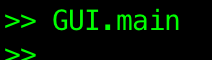
\includegraphics[width=0.2\textwidth]{0_1_startup}
 \caption{Type GUI.main and then press enter to launch ANACONDA2 GUI.}\label{0_1_startup}
\end{figure}

\clearpage
\subsection*{ANACONDA2 GUI overview}
\begin{wrapfigure}{r}{0.3\textwidth}
\centering
  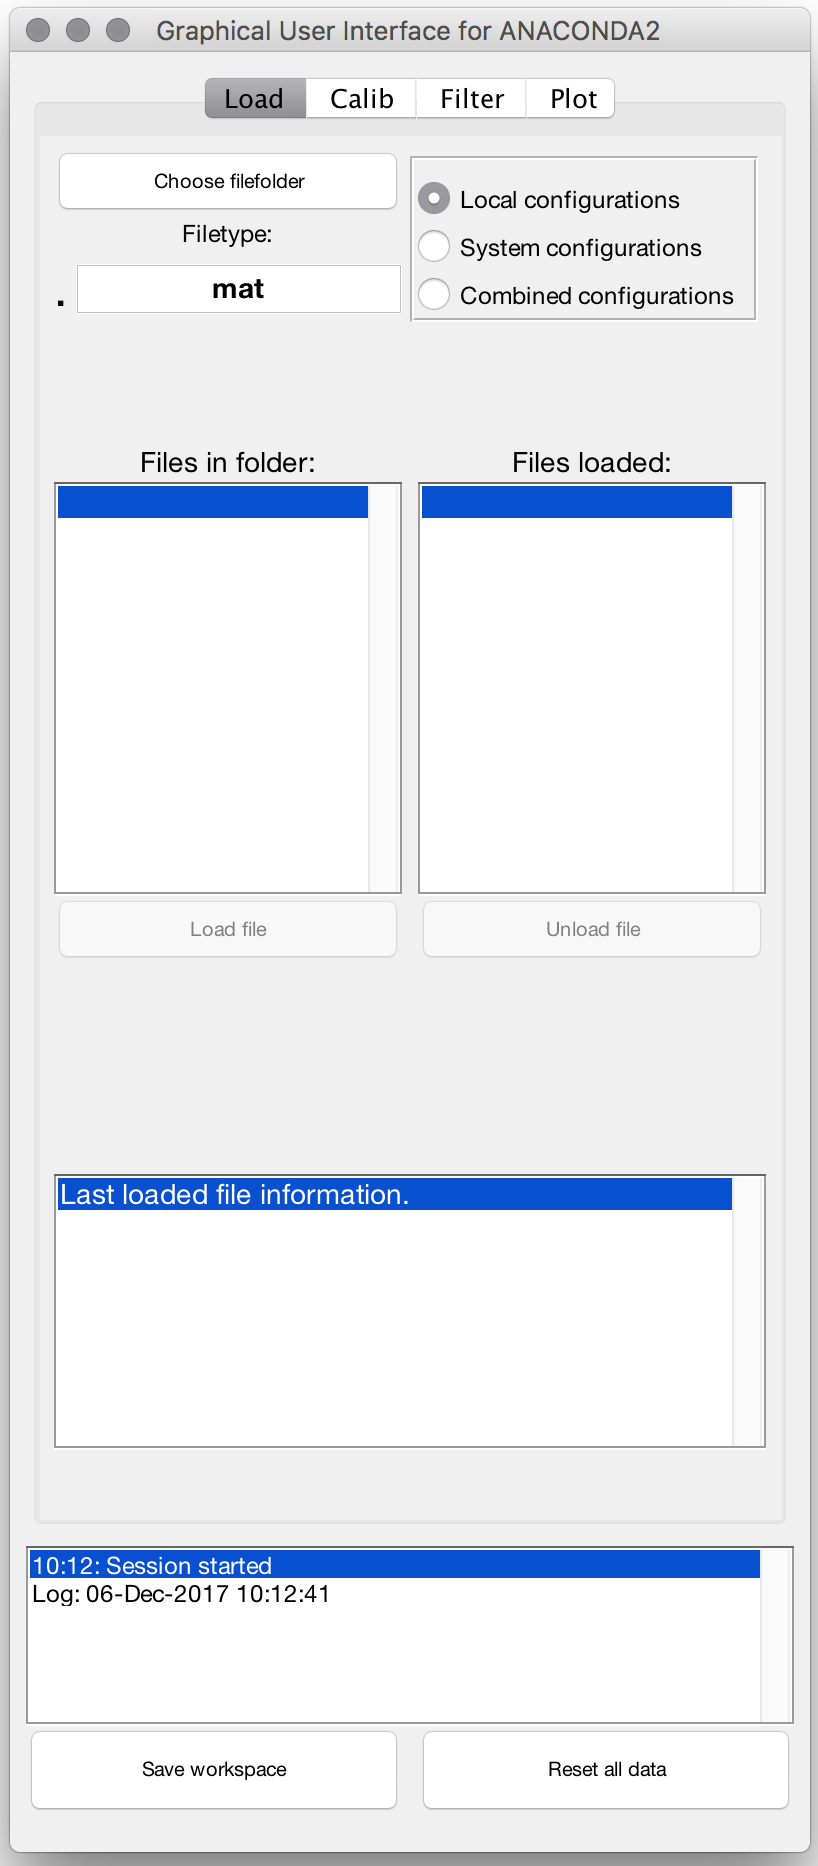
\includegraphics[width=0.3\textwidth]{1_1_startup}
 \caption{The start screen when launching the ANACONDA2 GUI.}\label{1_1_startup}
\end{wrapfigure}
When launching the ANACONDA2 GUI, the screen will look similar to Figure~\ref{1_1_startup}. There are four tabs, each representing a different part of the data treatment process in a chronological order.\\
\\
The first tab is a file handler tab, labelled as 'Load' since this is where files are loaded (resp. unloaded).\\
\\
The second tab is a calibration tab, labelled as 'Calib', where raw data files coming directly from experiments can be calibrated via multiple calibration procedures.\\
\\
The third tab is a filter tab in which data filters can be constructed, edited, removed and combined.\\
\\
The fourth tab is the plot tab, in which data can be plotted and where new plot- and signal configurations can be created.\\
\\
On the bottom, there is a big window which is the 'log box'. In it, the different actions performed with the GUI can be found.\\
\\
Reset all data means that the GUI will restart and all work will be deleted.\\
\\
Save workspace means that all files that have been loaded will have their respective metadata files replaced or stored in their respective location.

\clearpage
\section*{Data treatment part 1: File Handler}
\begin{figure}[h]
\centering
  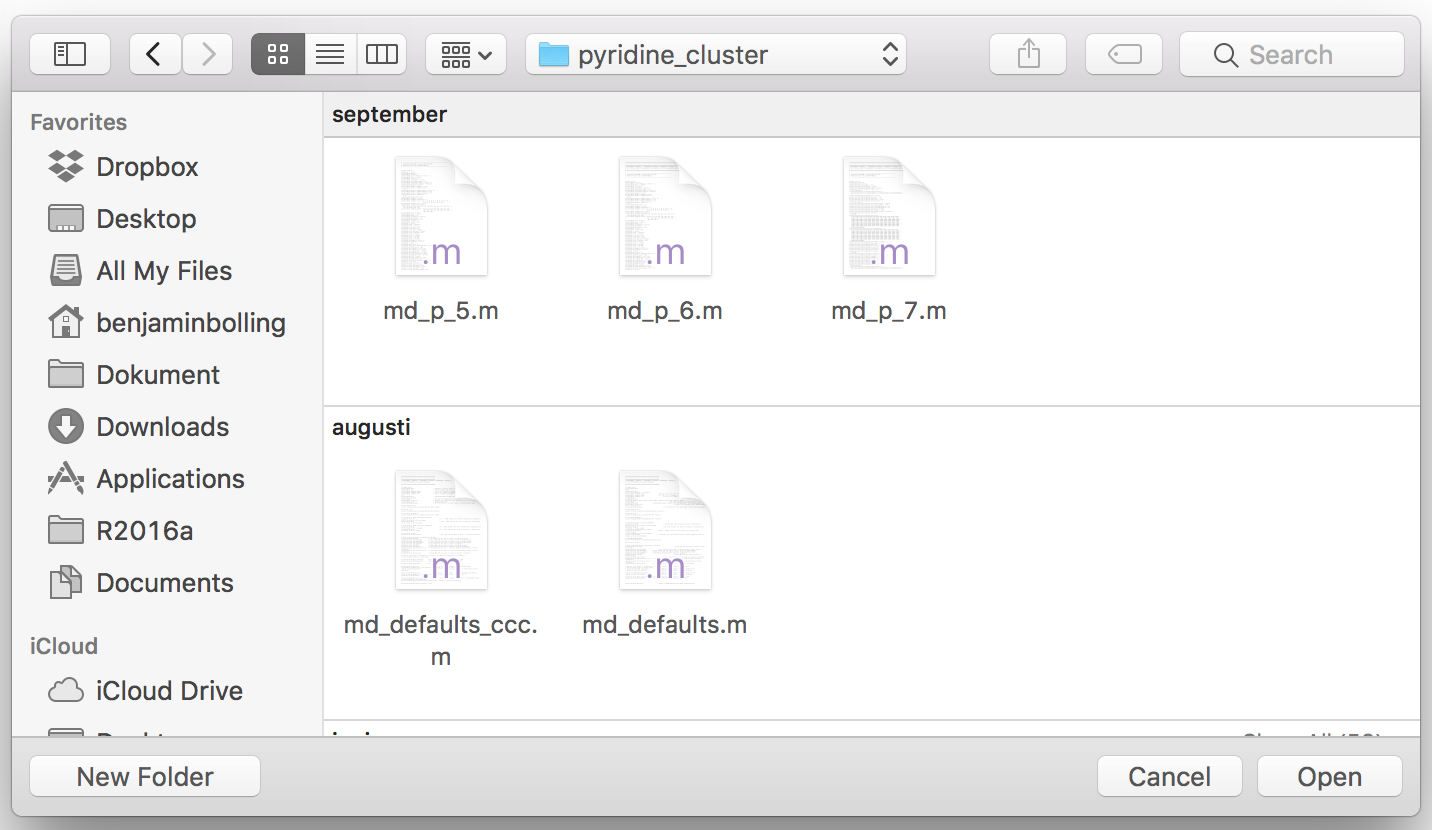
\includegraphics[width=0.4\textwidth]{1_2_choosefolder}
 \caption{Browse into the folder where the experimental data files are located.}\label{1_2_choosefolder}
\end{figure}
To load data files, they have to be in one of the following filetypes: .dlt, .mat.\\
\begin{wrapfigure}{r}{0.3\textwidth}
\centering
  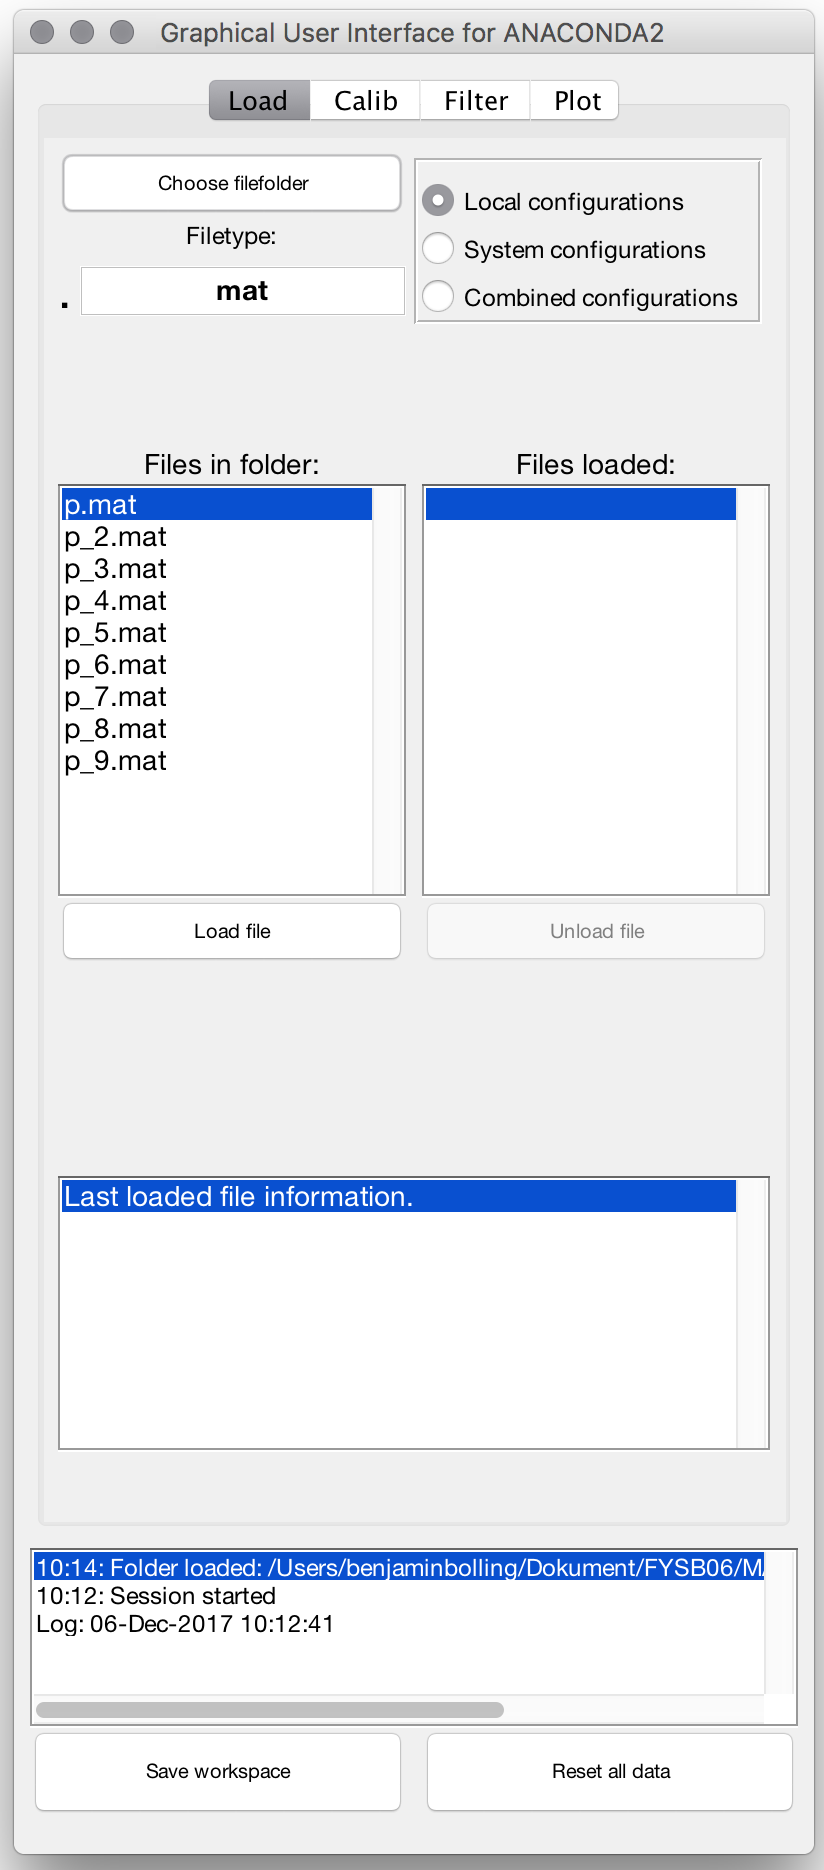
\includegraphics[width=0.3\textwidth]{1_3_choosefile}
 \caption{Files in selected folders with selected filetype can be seen.}\label{1_3_choosefile}
\end{wrapfigure}
In order to get the files from an experiment, click on 'Choose filefolder' and browse into the folder where the experimental data files are located and press 'Open'. Once opened, the filehandler will show all files with the selected file-extension (e.g. '.mat' as seen in Figure~\ref{1_3_choosefile}) in the folder. The filetype can be edited by simply clicking in the box and writing another file-extension, e.g. '.dlt', and pressing enter or with the mouse anywhere outside the box. This will result in that all '.dlt'-files in the folder will be shown.\\
Before loading a file, the load configurations should be selected which describes how a file is to be loaded.
\begin{itemize}
\item'Local configurations' selected means that if there is a readable configuration file in the same folder with the name 'md\_[filename].m', this file will be used when the [filename] data file is loaded.
\item'System configurations' means that a pre-defined spectrometer can be selected in order to generate the metadata necessary for the data treatment.
\item'Combined configurations' means that both local and system configurations will be used. If any overlap is found for a metadata, the metadata defined in local configurations will be used.
\end{itemize}
\clearpage
\begin{figure}[h]
\centering
  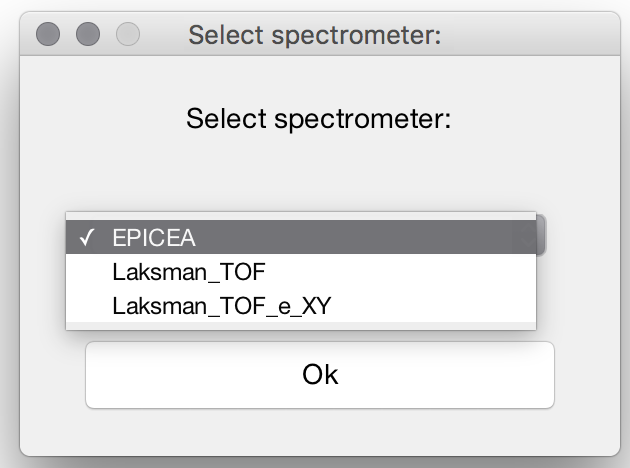
\includegraphics[width=0.4\textwidth]{1_4_loadfile_specset}
 \caption{When using system configurations to load a file, there are three spectrometers that can be chosen from.}\label{1_4_loadfile_specset}
\end{figure}
\begin{wrapfigure}{r}{0.3\textwidth}
\centering
  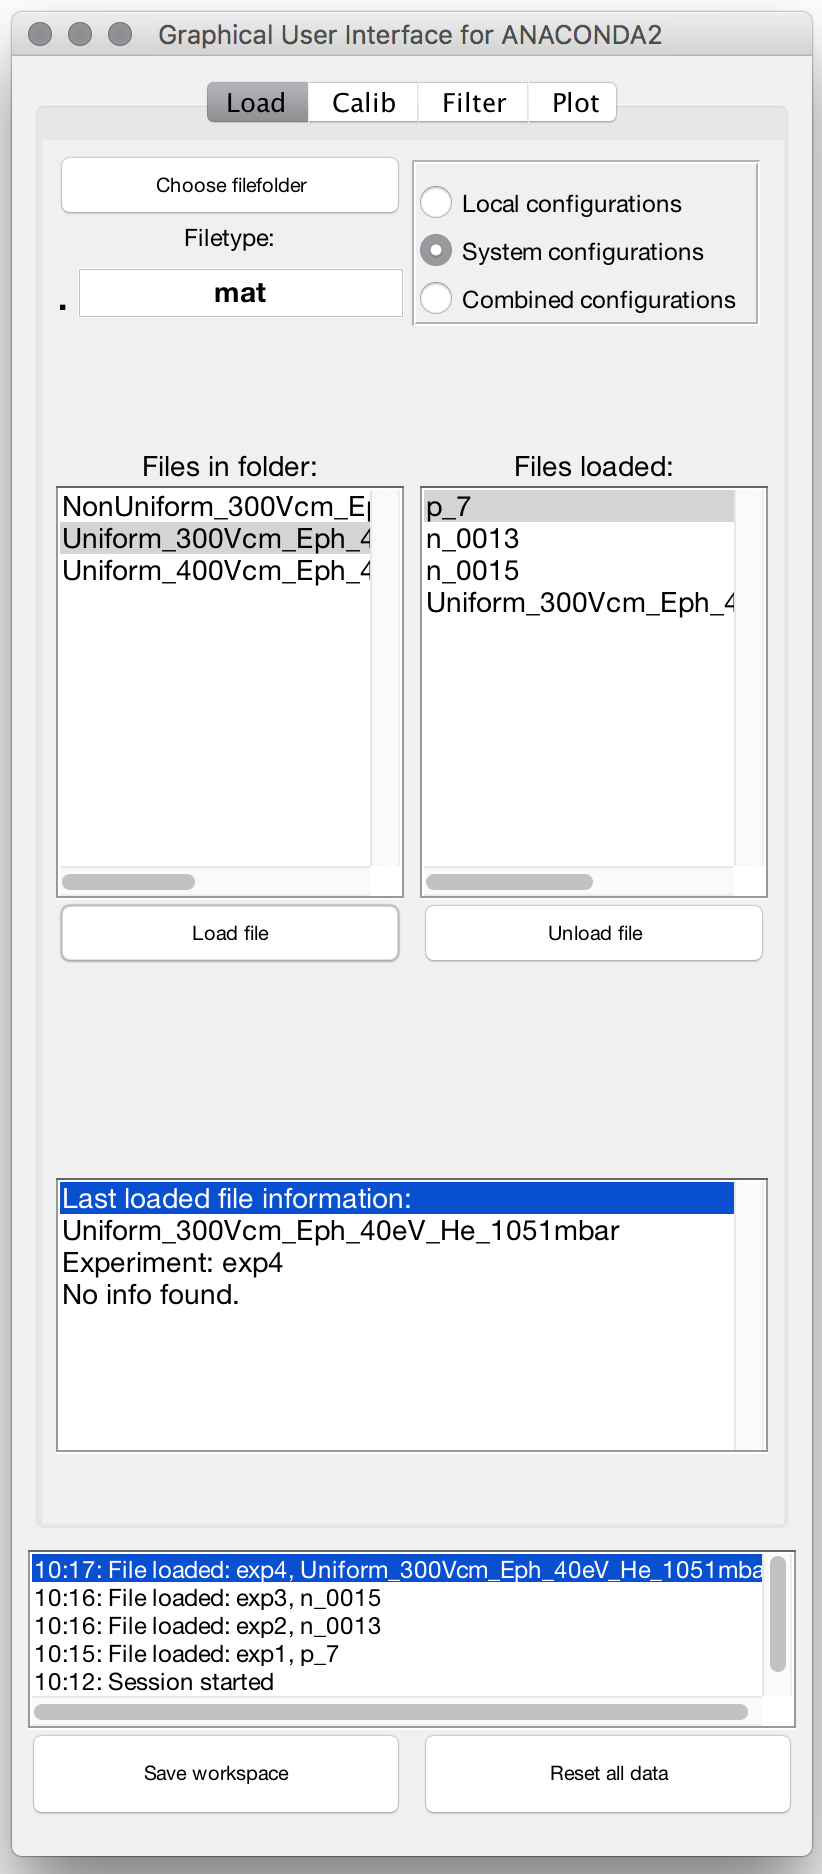
\includegraphics[width=0.3\textwidth]{1_5_filesloaded}
 \caption{Files in selected folders with selected filetype can be seen.}\label{1_5_filesloaded}
\end{wrapfigure}
There are currently three available spectrometers: EPICEA, Laksman\_TOF and Laksman\_TOF\_e\_XY. Their properties and differences can be found in...\\% References. EPICEA is a spectrometer at SOLEIL.
%Rename Laksman_TOF_e_XY to Oostenrijk_2D and Laksman_TOF to Laksman_3D.
\\
To load the selected file, press 'Load file' after having selected the desired configurations. As files are being loaded into memory, they will be visible in the 'Files loaded'-list. The last loaded file's information will be shown in the file information window, which exists if it has been properly defined during data acquisition during an experiment. Selecting a loaded file results in that this file's information will be shown in the file information window.\\
\\
To unload a file from memory, select a loaded file and press 'Unload file'.\\
\\
In our example, we have loaded 4 different data files from 3 different experiments, stored at three different locations. The first three files have been loaded using local configurations whilst the last file was loaded with system configurations with the Laksman\_TOF\_e\_XY spectrometer.

\clearpage
\section*{Data treatment part 2: Data Calibration}
[ EMPTY FOR NOW�- NOT YET CONSTRUCTED. ]

\clearpage
\section*{Data treatment part 3: Data Filters}
\begin{wrapfigure}{r}{0.3\textwidth}
\centering
  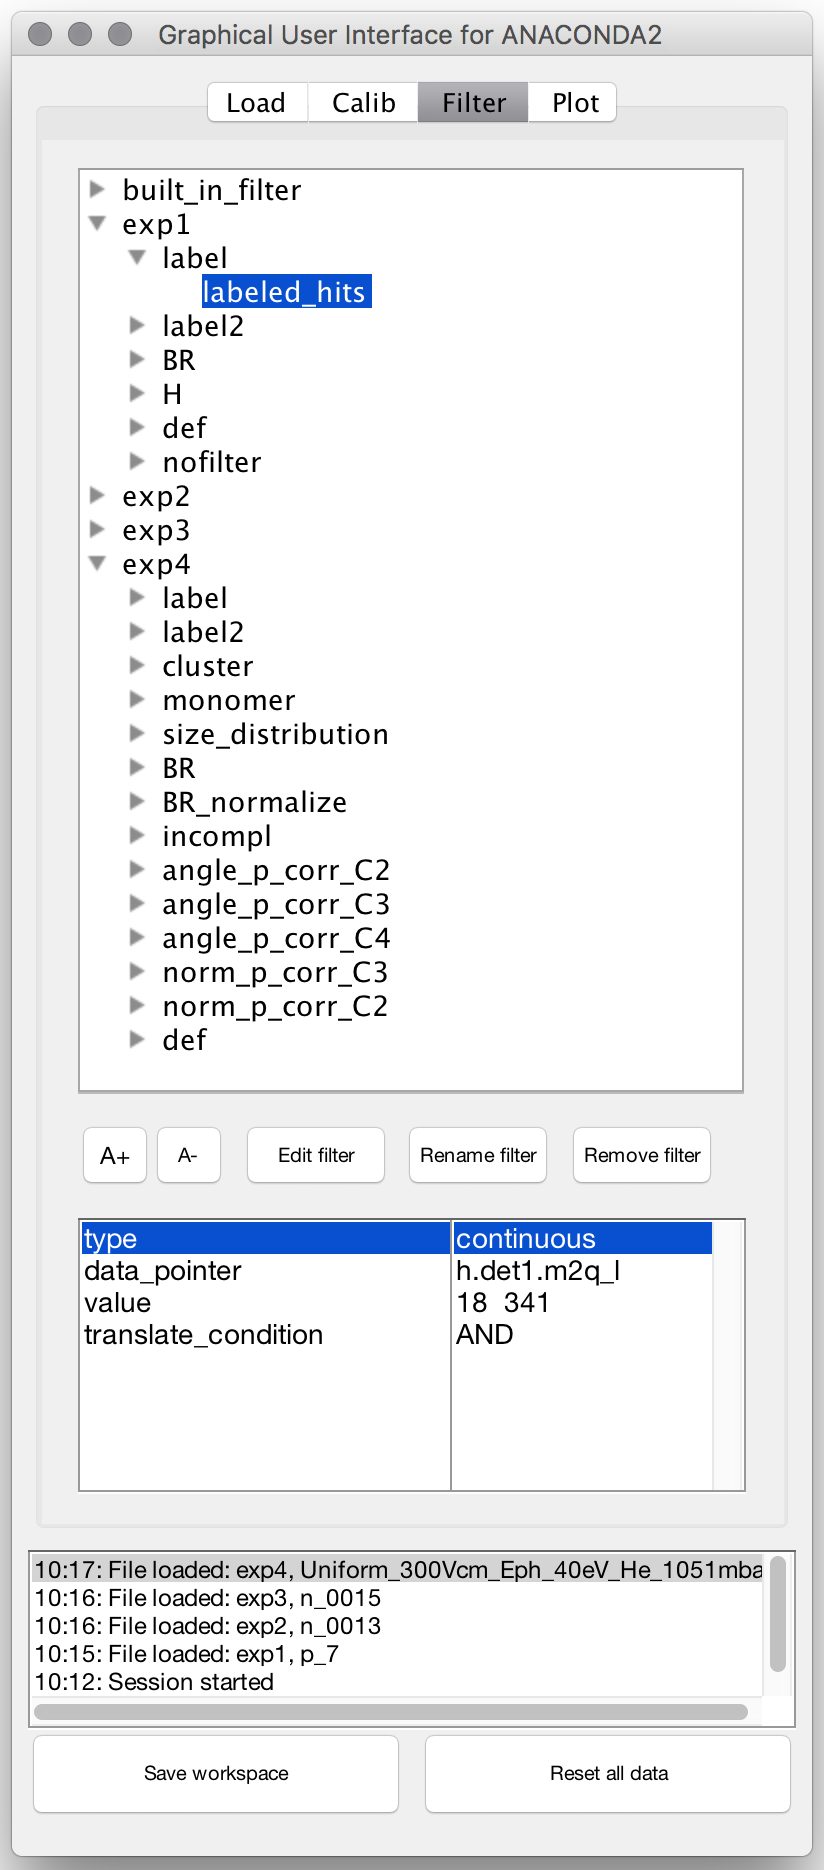
\includegraphics[width=0.3\textwidth]{3_1_filter_sel}
 \caption{The filter tab.}\label{3_1_filter_sel}
\end{wrapfigure}
The actions that can be done with data filters is the following: Construction of new filters, editing filters, renaming filters and removing filters. The fontsize of the filters can be increased resp. decreased by clicking on A+ resp. A-.\\
\\
By opening up the tree of data filters for the different experiments, selecting a filter results in that all its conditions will be shown. If a combined filter is selected, the operator of the combined filter will be shown. If no operator has been defined, the standard condition 'AND' will be shown as operator. To edit a field, double-click on the field to edit, which opens up a window with the previous value (Figure~\ref{3_2_filter_cond_edit}) that can be edited and stored by pressing 'Ok'.\\
\\ %Introduce concept of a recursive filter. What is a combined filter? What is an operator? 
To construct a new filter, select one of the built-in filters or the built-in combined filter, and drag-and-drop it to the desired experiment. The parameters can then be edited. Note that filters can also be drag-and-dropped between different experiments.\\
\\
To rename a filter, press the 'Rename' button and type in the desired name. Note that the name has to start with a letter, and there cannot be any spaces or blanks - in these cases, use the underscore symbol.
\begin{figure}[h]
\centering
  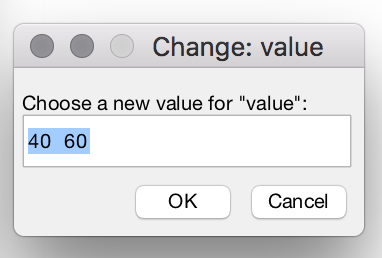
\includegraphics[width=0.3\textwidth]{3_2_filter_cond_edit}
 \caption{The 'Value' of the 'labeled\_hits' filter ie being edited.}\label{3_2_filter_cond_edit}
\end{figure}
\clearpage
\begin{figure}[h]
\centering
  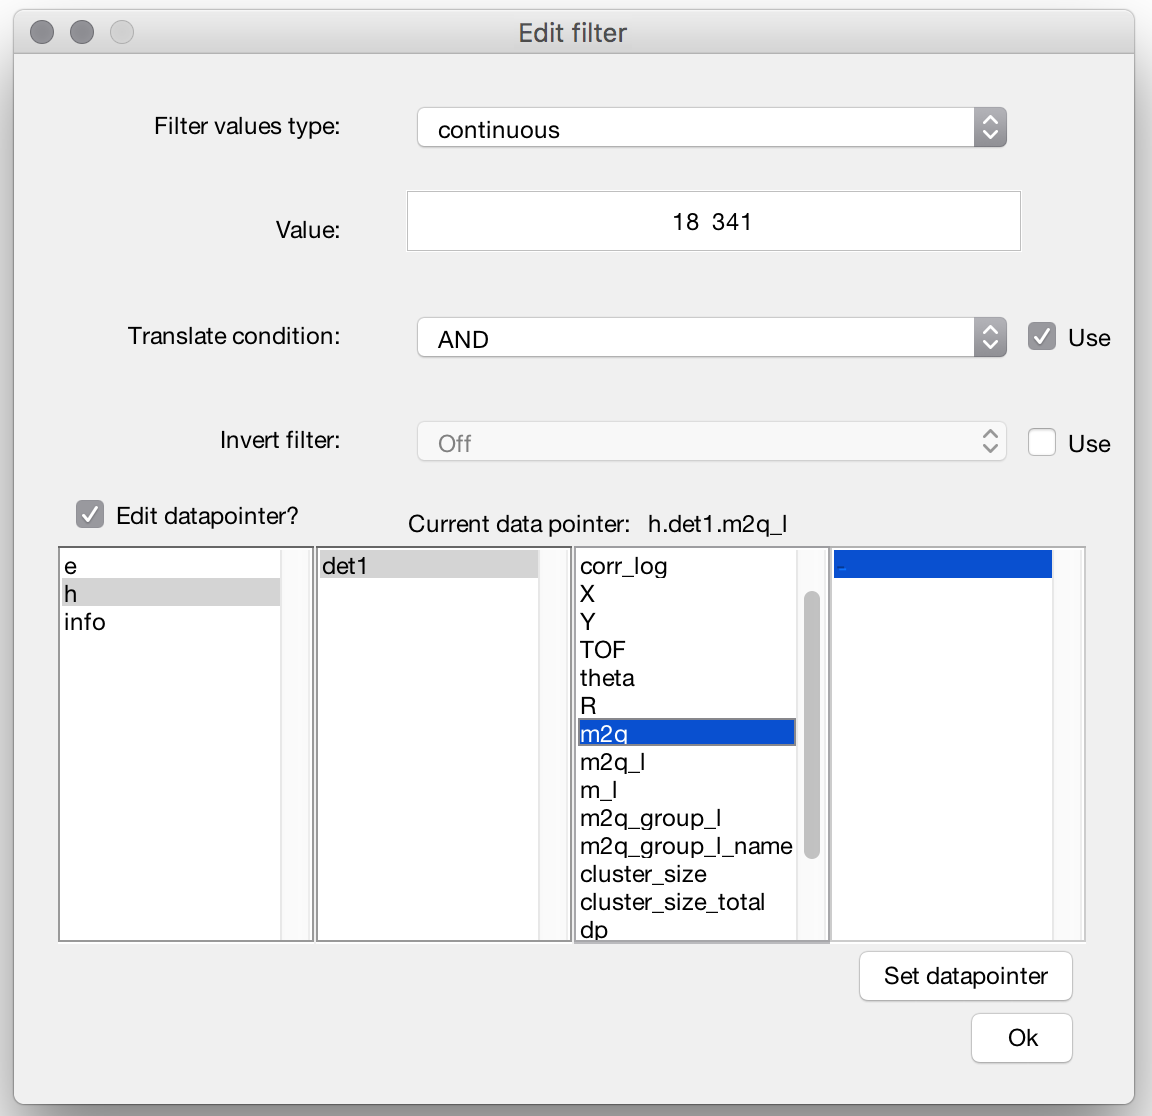
\includegraphics[width=0.8\textwidth]{3_3_filter_edit}
 \caption{Edit all fields of a filter by opening up the 'Edit filter' window.}\label{3_3_filter_edit}
\end{figure}
To fully edit all conditions of a (single, not combined) filter, select a filter and press the edit button. This results in that the 'Edit filter'-window will open up for the selected filter (Figure~\ref{3_3_filter_edit}), in which the filter value type can be selected, the values can be defined, translate condition can be defined or turned on or off, invert filter can be turned on or off, and data-pointer can be edited.\\
\\ % What is a data pointer?
The data pointer points towards a signal, and hence, the edit feature of the data pointer has been constructed such that the user can select signal that the data pointer points towards by using pre-defined signals in the 'Edit filter' window.\footnote{More advanced users can have it completely editable as a text string by double-clicking the data-pointer field without opening the 'Edit filter' window, e.g. for a mathematical formula (e.g. "exp.h.det1.KER/3").}

\clearpage
\section*{Data treatment part 4: Plotting}
% Make a flowchart figure of the making of a plot. Signal + metadata + filter have to be defined. Filter goes into metadata. External filters overwrite internal.
The last part of data treatment is to plot the data. The first step is to select experiments which are to be plotted (multi-selection is available). Then select filter to apply to the experiment, followed by plot type. The pre-defined plots has two different sections: Built-in and customized plots. The built-in plots are hard-coded and loaded as standard plot types with the experiment during load, whilst the customized plots are the plots that have been constructed by the user in 'New plot conf'.
\begin{figure}[h]
\centering
  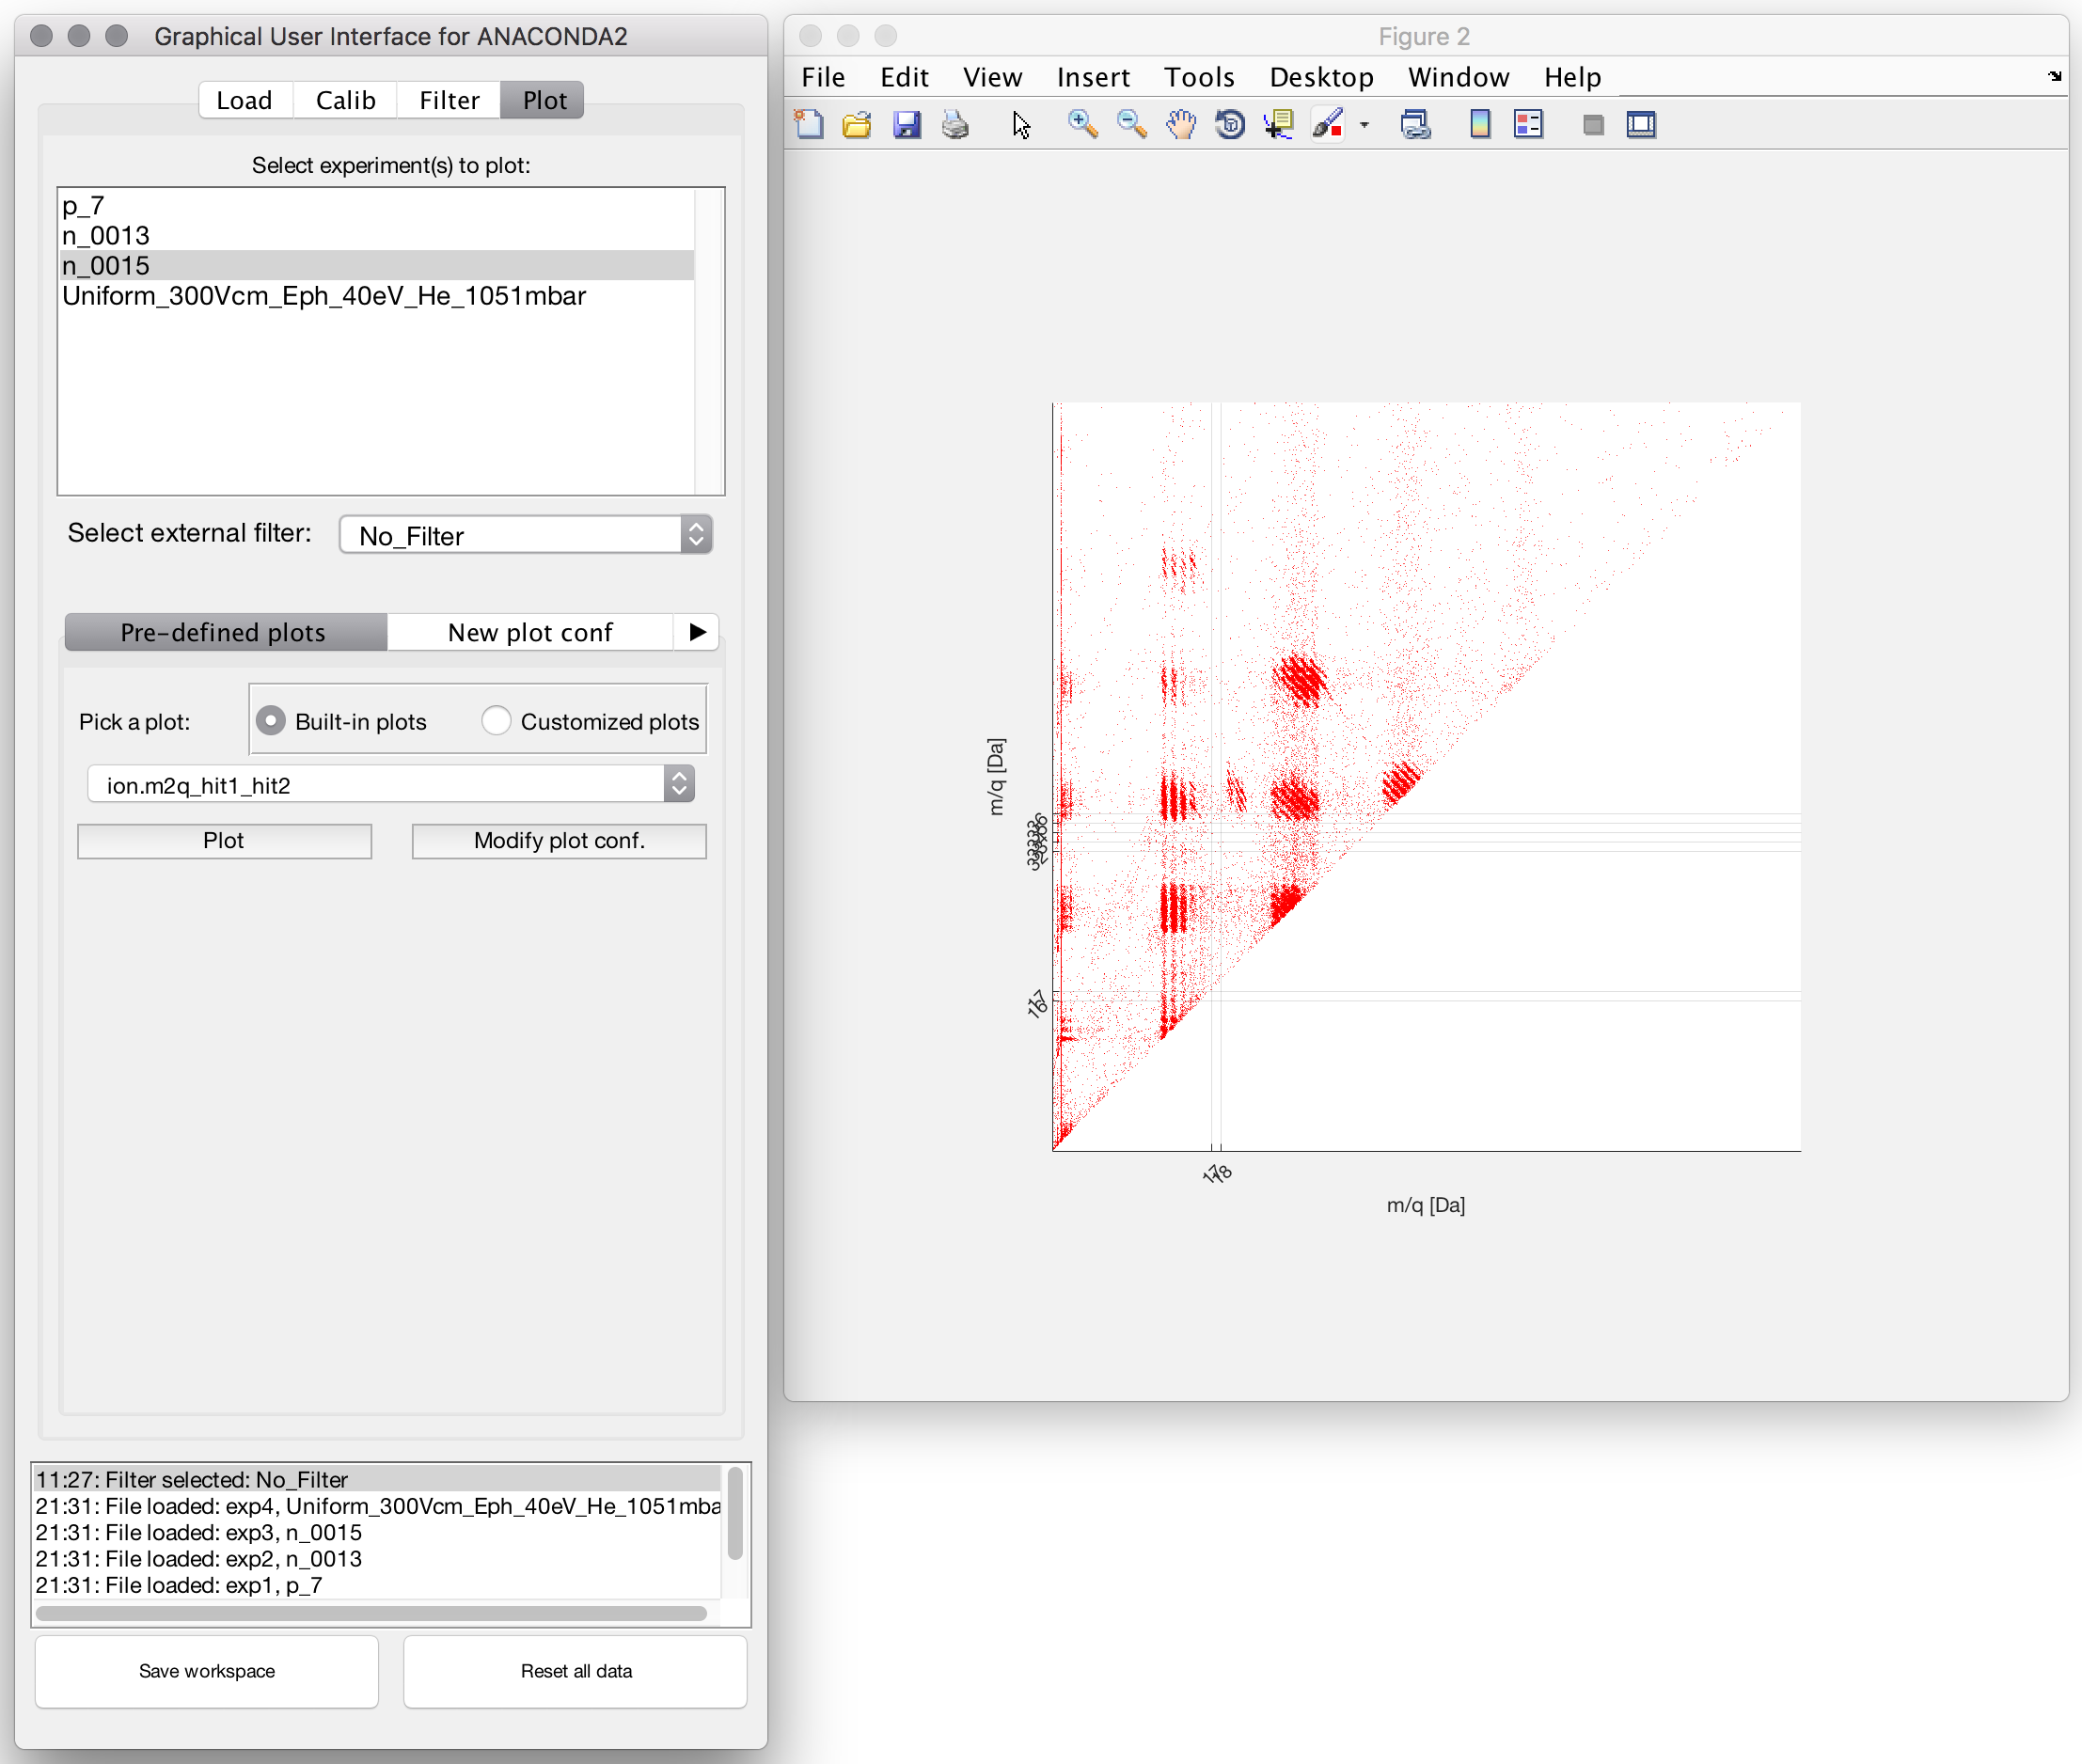
\includegraphics[width=0.8\textwidth]{4_1_plot_no_filter}
 \caption{A PEPIPICO plot for an ion-ion coincidence experiment with pyridine, with no filters applied.}\label{4_1_plot_no_filter}
\end{figure}
\clearpage
In order to construct new plot configurations, select a signal and put it as Ordinate ('X') or Abscissa ('Y'). In order to use something else than intensity as abscissa, click the checkbox for Abscissa. In Figure~\ref{4_4_plot_new_conf}, we have chosen to create a new plot where the radius R has been plotted as Abscissa against TOF (time-of-flight) as Ordinate.
\begin{figure}[h]
\centering
  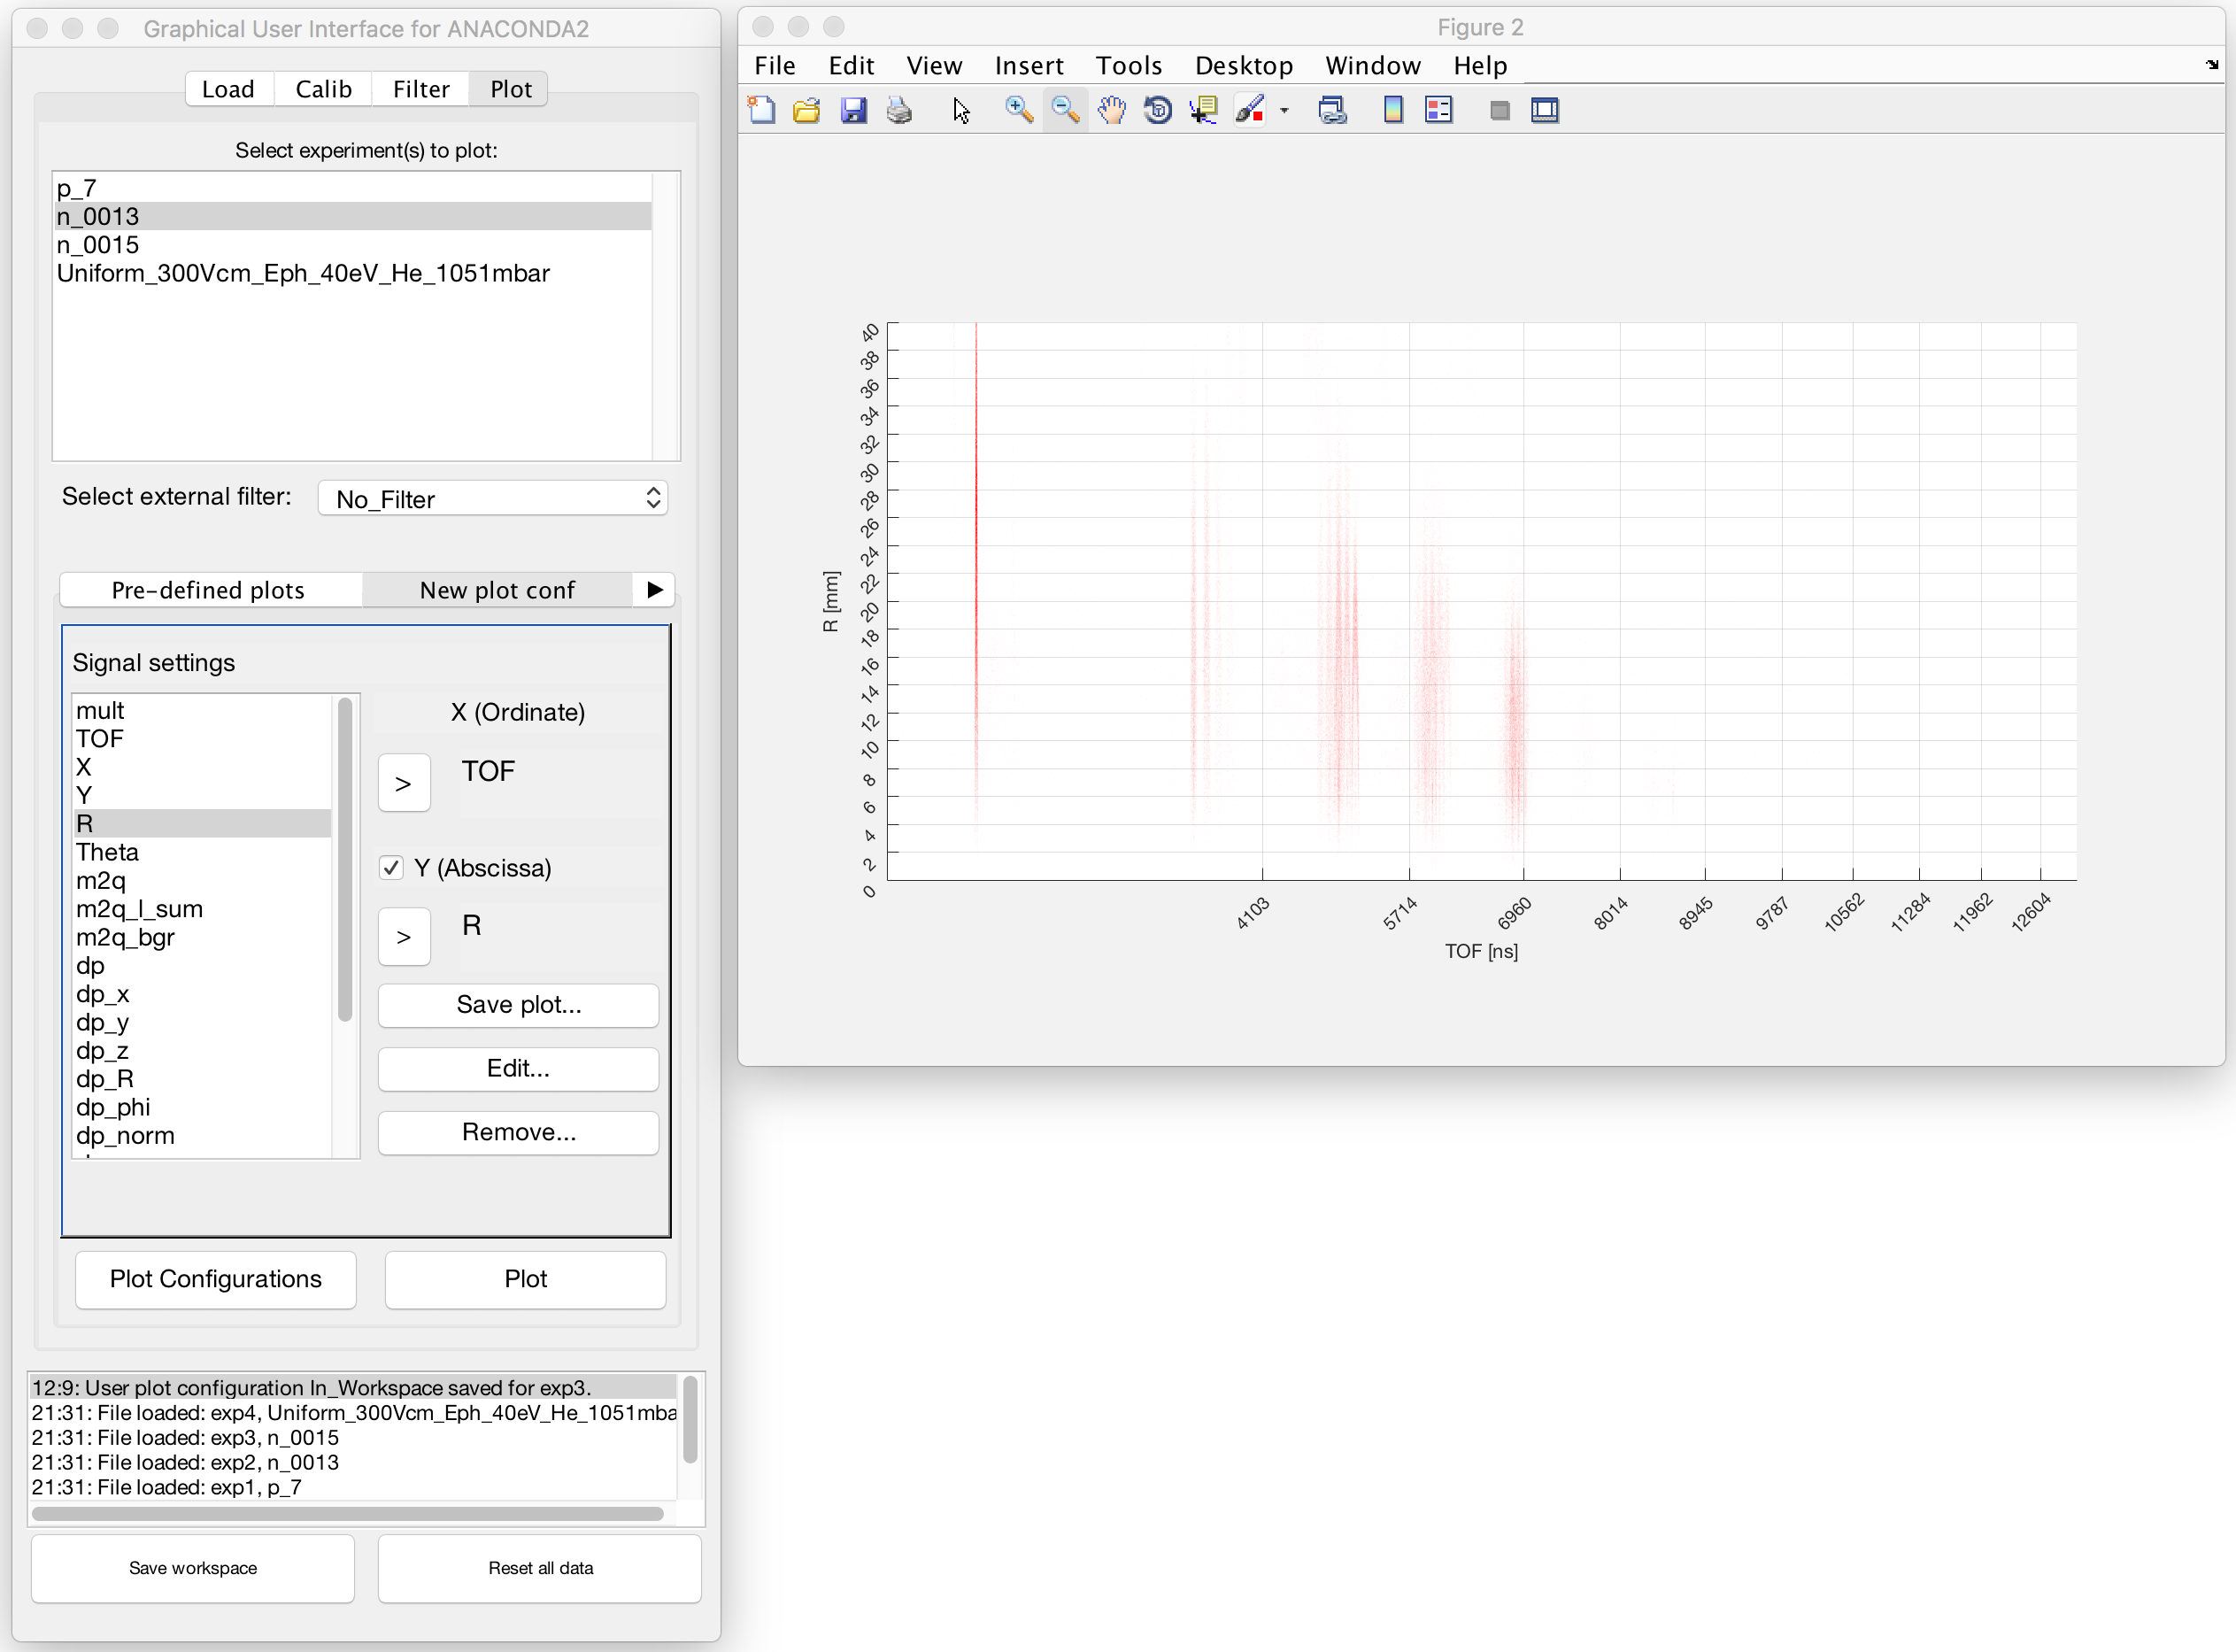
\includegraphics[width=0.8\textwidth]{4_4_plot_new_conf}
 \caption{A new plot configuration plotted: Radius R as abscissa vs. TOF (time-of-flight) as ordinate.}\label{4_4_plot_new_conf}
\end{figure}

\clearpage
\section*{Data treatment part 5: Data analysis}
Once all plots have been constructed, the next step is data analysis...\\
\\
In order to demonstrate how data can be selected by using various data filters, the same experiment was plotted three times with different filter conditions. In Figure~\ref{4_1_plot_no_filter}, Figure~\ref{4_2_plot_hits_filter} and Figure~\ref{4_3_plot_hits_events_filter}, the same PEPIPICO plot was created. In Figure~\ref{4_1_plot_no_filter}, no filters were applied. In Figure~\ref{4_2_plot_hits_filter}, a hits filter was applied, and in Figure~\ref{4_3_plot_hits_events_filter}, a combined filter was applied.
\begin{figure}[h]
\centering
  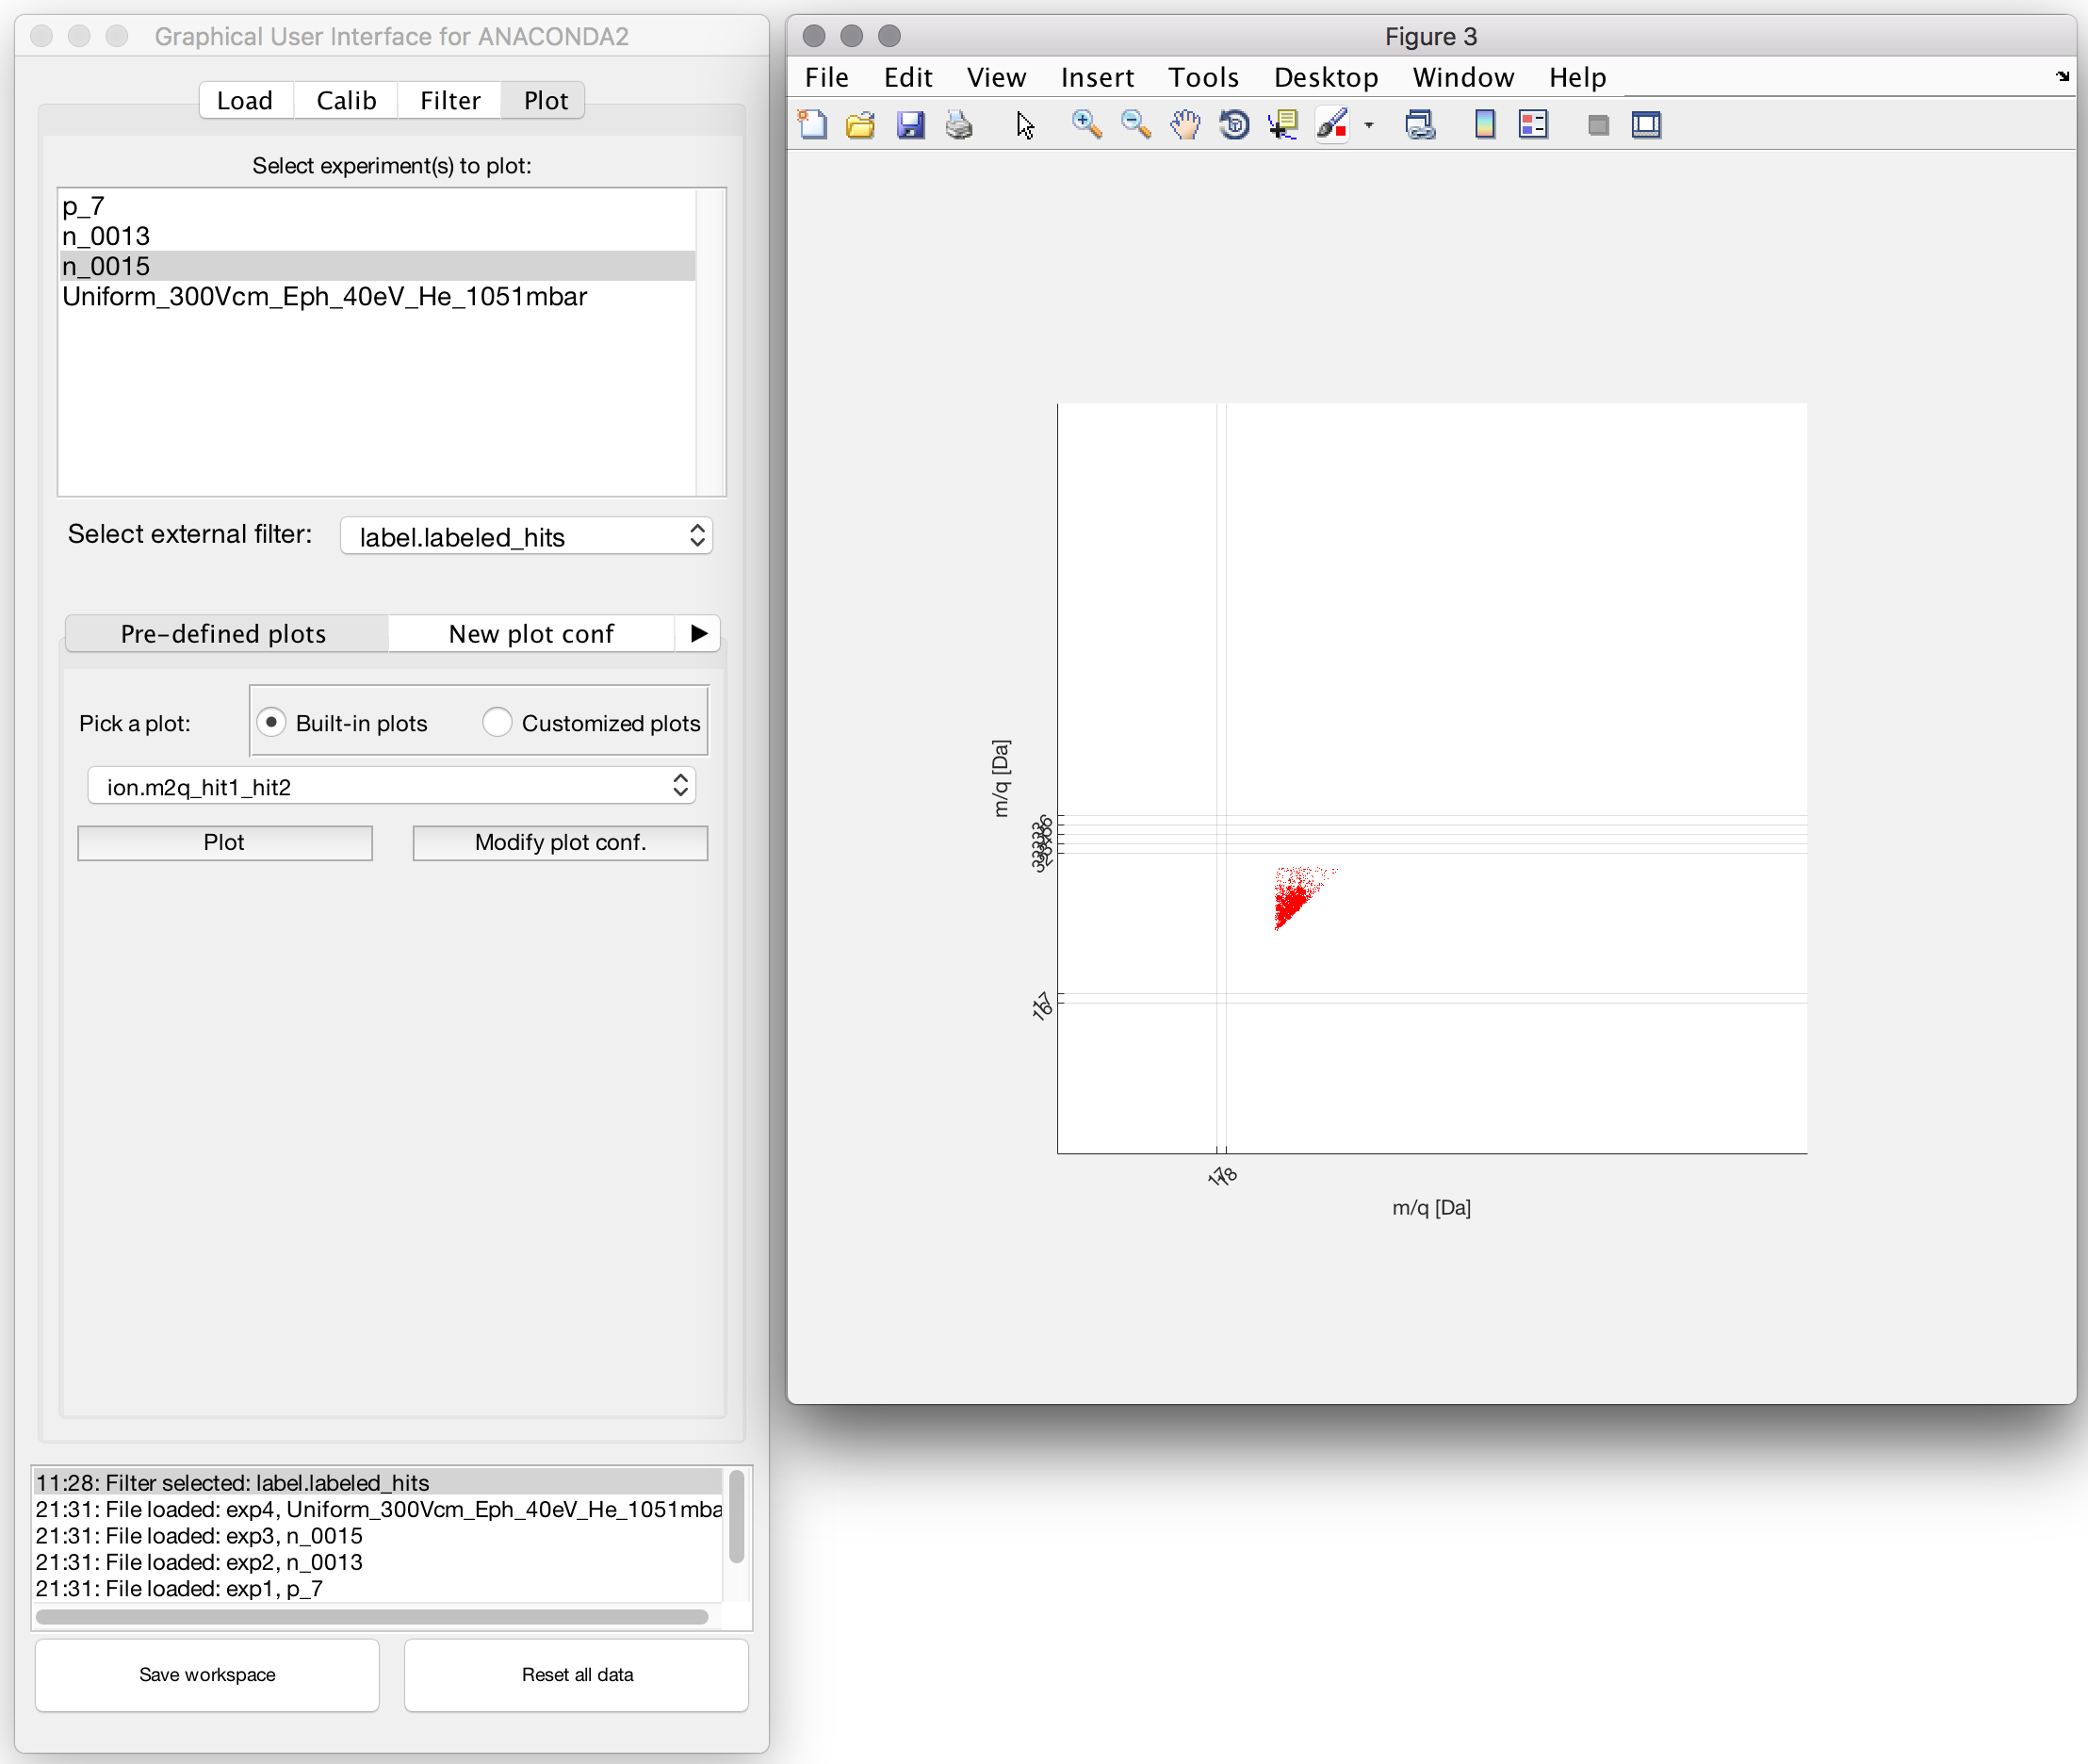
\includegraphics[width=0.6\textwidth]{4_2_plot_hits_filter}
 \caption{A PEPIPICO plot for an ion-ion coincidence experiment with pyridine, with a hits filter applied.}\label{4_2_plot_hits_filter}
\end{figure}
\begin{figure}[h]
\centering
  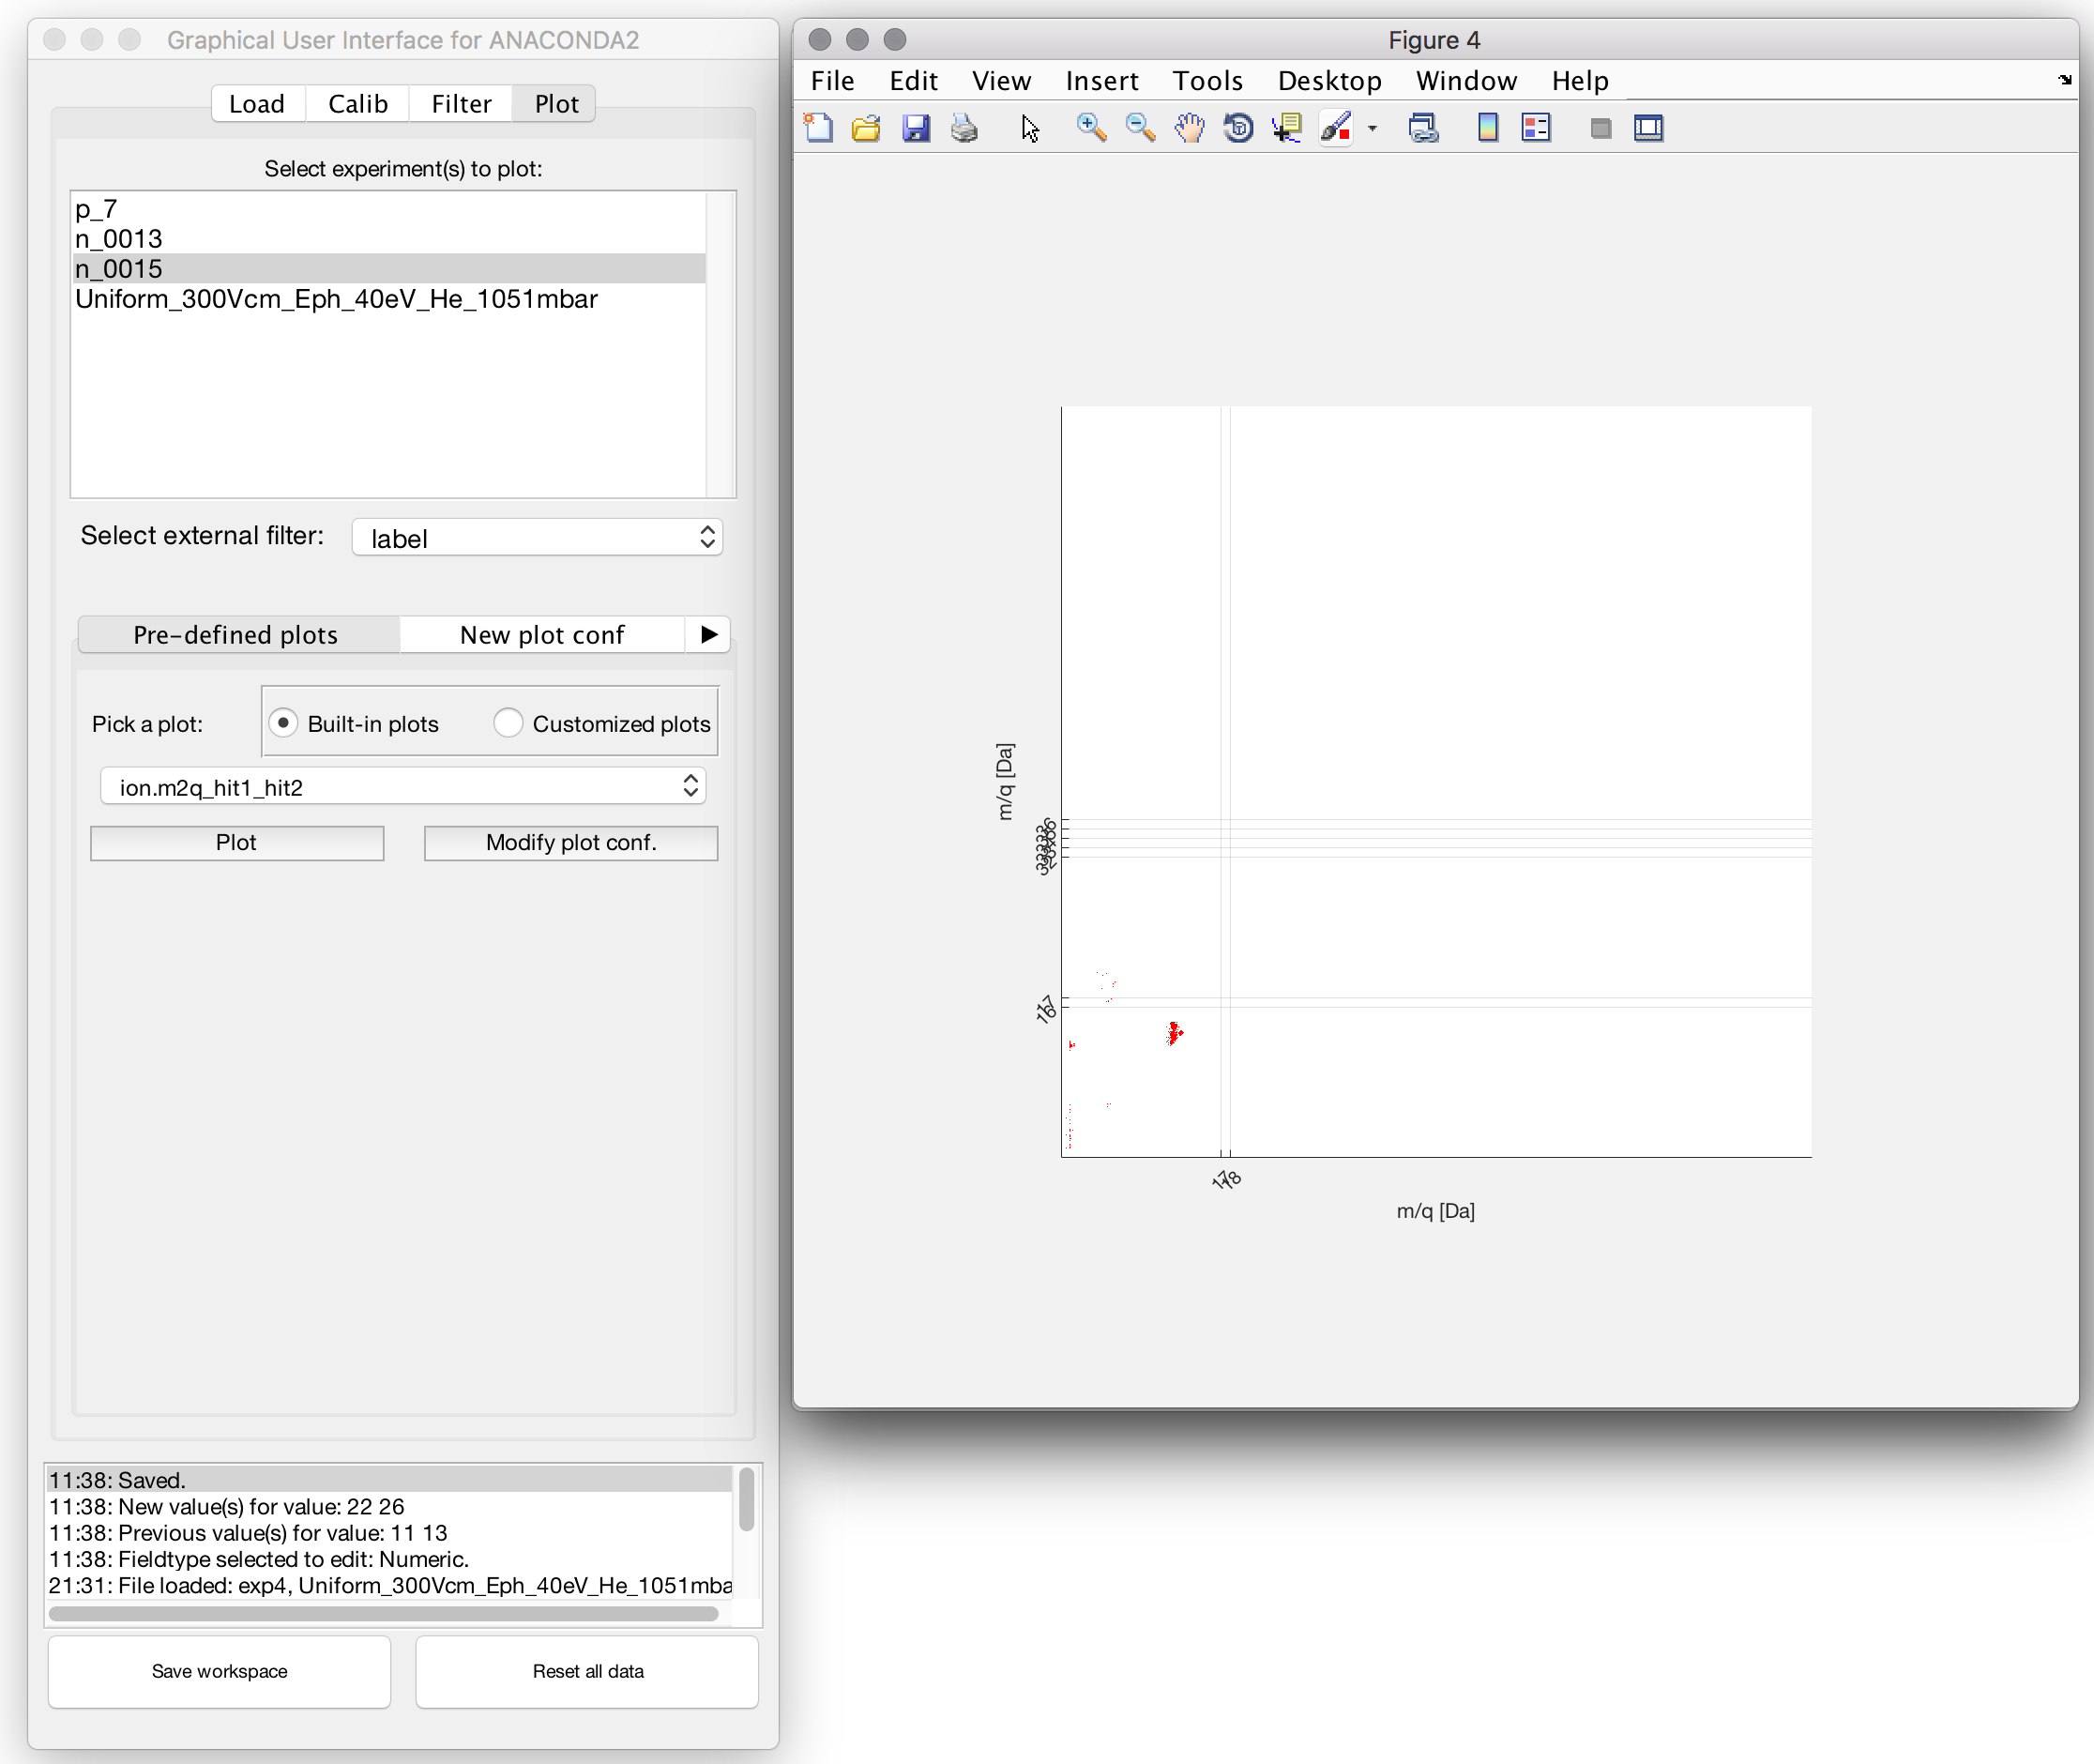
\includegraphics[width=0.6\textwidth]{4_3_plot_hits_events_filter}
 \caption{A PEPIPICO plot for an ion-ion coincidence experiment with pyridine, with a combined filter applied.}\label{4_3_plot_hits_events_filter}
\end{figure}

\clearpage
\section*{Table ...}
Table showing the meaning of e.g. m2q, m2q\_l

\clearpage
\section*{References}
\begin{thebibliography}{9}

\bibitem{Bart_Documentation}
  Bart Oostenrijk,
  \textit{Description of the Coincidence data analysis software},
  Department of Physics at Lund University,
  2nd edition,
  2018.

\end{thebibliography}


\end{document}











